\section{正则化与模型选择}
假设我们为了一个学习问题而在多个不同的模型之间做选择。比如,我们要用到多项式回归模型$h_\theta(x)=g(\theta_0,\theta_1x+\cdots,+\theta_kx_k)$,想要确定$k$是应该取$0,\cdots,10$种的一个。我们应该如何自动的选择模型,使其对偏差和方差有好的权衡?

假设我们有有限个模型$\mathcal{M}=\{M_1,\cdots,M_d\}$,我们尝试在其中选取。比如,在上面的模型中,模型$M_i$则表示$i$次的多项式回归模型。如果我们想在SVM,神经网络和逻辑斯蒂回归中选一个,则$\mathcal{M}$是包含这些模型的。

\subsection{交叉验证}
对于给定的训练集$S$,下面的想法是基于ERM的模型选择
\begin{enumerate}[1]
\item 在$S$上训练每个模型$M_i$,得到假设$h_i$
\item 选择有最小训练误差的假设
\end{enumerate}

这个算法不可行,考虑多项式模型,多项式次数越高,则其拟合训练集$S$的效果越好(训练误差越小),因此这种方法倾向于选择高方差的高次的多项式模型。
\subsubsection{留出交叉验证}
下面的方法有所改进。采用留出交叉验证法(hold-out cross validation)(或称为简单交叉验证(simple cross validation)),如下
\begin{enumerate}[1]
\item 随机地将$S$分割成$S_{train}$($70\%$的数据)和$S_{cv}$($30\%$的数据),$S_{cv}$被称为留出交叉验证数据集
\item 用$S_{train}$训练每一个模型$M_i$,得到假设$h_i$
\item 选择在留出交叉验证数据集上误差$\hat{\epsilon}_{S_{cv}}(h_i)$上最小的假设$h_i$。其中,$\hat{\epsilon}_{S_{cv}}(h_i)$指$h$在$S_{cv}$上的训练误差。
\end{enumerate}
一般情况下,留出交叉验证数据集选择数据的$\frac{1}{4}\sim\frac{1}{3}$,$30\%$是通常的选择。事实上,对于第三步,可以修改为在选出了$M_i$之后,再用完整的训练集$S$去训练。

\subsubsection{k折交叉验证}
留出交叉验证法的一个缺点是会“浪费”$30\%$的数据,即使我们有利用这部分数据对所选出来的$M_i$进行再训练,但是只是用了$70\%$的数据来,于是就有如下的算法:k折交叉验证(k-fold cross validation)
\begin{enumerate}[1]
\item 将数据集$S$分割成$k$个不想交的子集,每个子集包含$\frac{k}{m}$个数据,将其记为$S_i,i=1,2,\cdots,k$
\item for $j=1,\cdots,k$\\
\indent\ \ 在数据集$S_1\cup\cdots\cup S_{j-1}\cup S_{j+1}\cup\cdots\cup S_k$得到假设$h_{ij}$,并计算$h_{ij}$在$S_j$上的误差$\hat{\epsilon}_{S_j}(h_{ij})$\\
\indent\ \ 对$\hat{\epsilon}_{S_j}(h_{ij})$在$j$上求均值,得到模型$M_i$上的泛化误差估计值。
\item 选择具有最小的泛化误差模型$M_i$,然后用完整的数据集$S$来重新训练$M_i$。
\end{enumerate}
一种典型的选择是将$k$设为10,虽然数据的比率变为了$\frac{1}{k}$,比以前少很多,而且计算的复杂度也比留出交叉验证要大,因为需要对每个模型训练$k$次。
\subsubsection{留一交叉验证}
当数据量很匮乏时,可能会使用极端的方法:$k=m$。在这种情况下,模型将会在$m-1$的数据集中做训练,用剩下的一个数据做测试。最后也是通过对得到的$m$个模型做平均,得到模型的泛化误差估计值。这种模型称为留一交叉验证(leave-one-out cross validation)。

\subsubsection{自助法}
留一法受训练样本规模变化的影响较小,但计算复杂度又太高,一种方法在减少训练样本规模造成的影响,同时还能比较高效地进行实验估计。

“自助法”(bootstrapping)如下。给定包含$m$个样本的数据集$D$,我们对它进行采样产生数据集$D'$:每次随机从$D$中挑选一个样本,并将其拷贝如$D'$,然后将该样本放回初始数据集$D$中,使这个样本在下一次采样时还可能被采到,这个过程重复执行$m$次后,就得到了包含$m$个样本的数据集$D'$。$D$中有一部分样本会在$D'$中多次出现,而另一部分样本不出现。样本在$m$次采样中始终不被采到的概率时$(1=\frac{1}{m})^m$,取极限有
\begin{eqnarray}
\lim_{m\rightarrow\infty}\left( 1-\frac{1}{m} \right)^m=\frac{1}{e}\sim 0.368
\end{eqnarray}
即通过自主采样,初始数据集$D$中约有$36.8\%$的样本未出现在采样数据集$D'$中,因此可以将$D'$用作训练集,$D-D'$用作测试集。这样,实际评估的模型与期望评估的模型都使用了$m$个训练样本,而仍有数据总量约为$\frac{1}{3}$的没在训练集中出现的样本用于测试。这样的测试结果,称为“包外估计”(out-of-bag estimate)。

自助法在数据集较小、难以有效划分训练集和测试集时很有用,又自助法能从初始数据集中产生多个不同的训练集,这对集成学习等方法有很大的好处。然而,自助法产生的数据集改变了初始数据集的分布,这会引入估计误差。因而,当初始数据量足够时,其他交叉验证法更为常用。

\subsection{性能度量}
性能度量是衡量模型泛化能力的评价标准。在预测任务中,给定样例集$D=\{(\sample{x}{i},\sample{y}{1}),\cdots,(\sample{x}{m},\sample{y}{m})\}$,其中$\sample{y}{i}$是示例$\sample{x}{i}$的真实标记,要评估学习器$f$的性能,就要把学习器预测结果$f(x)$和真实标记$y$进行比较。 
\subsubsection{错误率与精度}
定义分类错误率为
\begin{eqnarray}
E(f;D)=\frac{1}{m}\sum_{i=1}^m 1(f(\sample{x}{i})\neq \sample{y}{i})
\end{eqnarray}
精度定义为
\begin{eqnarray}
acc(f;D)&=&\frac{1}{m}\sum_{i=1}^m 1(f(\sample{x}{i})= \sample{y}{i})\\
&=&1-E(f;D)
\end{eqnarray}
或对于数据分布$\mathcal{D}$和概率密度函数$p(x)$
\begin{eqnarray}
E(f;D)=\int_{x\sim D} 1(f(x)\neq y)p(x)dx
\end{eqnarray}
\begin{eqnarray}
acc(f;D)&=&\int_{x\sim D} 1(f(x)= y)p(x)dx\\
&=&1-E(f;D)
\end{eqnarray}
\subsubsection{查准率、查全率与F1}
对于二分类问题,将真实类别和预测类别的组合分为真正例(true positive),假正例(false positive),真反例(ture negative),假反例(false negative),分别记为$TP,FP,TN,FN$,显然有$TP+FP+TN+FN=$样例总数,定义混淆矩阵如下

\begin{center}
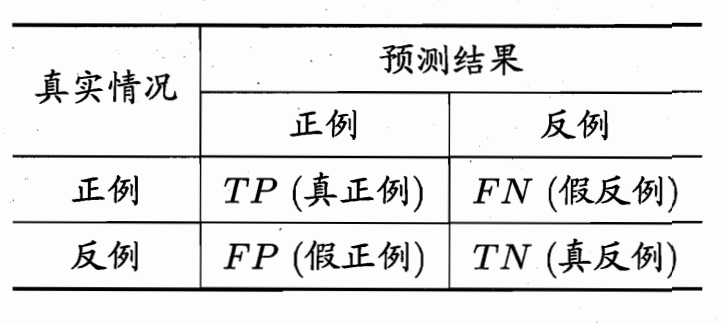
\includegraphics[scale=0.5]{../figures/RAMS1.PNG} 
\end{center}

查准率(也叫精度,precision)$P$与查全率(也叫召回率,recall)$R$定义为
\begin{eqnarray}
P=\frac{TP}{TP+FP}\\
R=\frac{TP}{TP+FN}
\end{eqnarray}
一般来说,查准率高时,查全率往往偏低,查全率高时,查准率往往偏低。

\paragraph{P-R曲线的绘制}对学习器的预测结果对样例进行排序,排在前面的是学习器认为“最可能”是正例的样本,排在最后的是学习器认为“最不可能”是正例的样本,按此顺序逐个把样本作为正例进行预测,则每次可以计算出当前的查全率、查准率,以查准率为纵轴,查全率为横轴作图,得到P-R曲线如下
\begin{center}
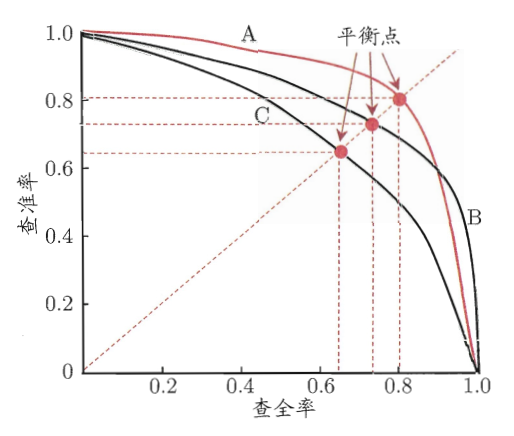
\includegraphics[scale=0.8]{../figures/RAMS2.PNG} 
\end{center}
若一个学习器的P-R曲线被另一个学习器的曲线完全“包住”,则可断言后者的性能优于前者。若两个学习器的P-R曲线有交叉点,则有以下的方法
\paragraph{平衡点(Break-Even Point,简称BEP)}它是“查准率=查全率”时的取值,如上图的学习器C的BEP为0.64,基于BEP的比较,认为学习器A优于B。
\paragraph{$F1$度量}BEP过于简化,通常用F1度量。F1是基于查准率与查全率的调和平均定义的
\begin{eqnarray}
\frac{1}{F1}=\frac{1}{2}\cdot(\frac{1}{P}+\frac{1}{R})
\end{eqnarray}
得到
\begin{eqnarray}
F1=\frac{2\times P\times R}{P+R}=\frac{2\times TP}{m+TP-TN}
\end{eqnarray}
其中,$m$为样例总数。
\paragraph{$F_\beta$度量}若对查准率和查全率重视程度不同,则用$F1$度量的一般形式:$F_\beta$,能让我们表达出对查准率、查全率的不同偏好,定义为
\begin{eqnarray}
F_\beta=\frac{(1+\beta^2)\times P\times R}{(\beta^2\times P)+R}
\end{eqnarray}
其中,$\beta>0$度量了查全率对查准率的相对重要性。$\beta=1$时退化为标准的$F1$,$\beta>1$时查全率有更大影响,$\beta<1$是查准率有更大影响。

很多时候会有多个混淆矩阵,有时进行多次的训练测试,或在多个数据集上进行训练测试,希望评估算法的“全局”性能,或是进行多分类任务。总之,是希望在$n$个二分类混淆矩阵上综合考察查准率和查全率。
\paragraph{宏查准率(macro-P)、宏查全率(macro-R)与宏F1(macro-F1)}先在各混淆矩阵上分别计算查准率和查全率,记为$(P_1,R_1),(P_2,R_2),\cdots,(P_n,R_n)$,再计算平均值
\begin{eqnarray}
macro-P&=&\frac{1}{n}\sum_{i=1}^nP_i\\
macro-R&=&\frac{1}{n}\sum_{i=1}^nR_i\\
macro-F1&=&\frac{2\times macro-P\times macro-R}{macro-P+macro-R}
\end{eqnarray}
\paragraph{微查准率(micro-P)、微查全率(micro-R)与微F1(micro-F1)}先在各混淆矩阵上分别计算查准率和查全率,记为$(P_1,R_1),(P_2,R_2),\cdots,(P_n,R_n)$,对混淆矩阵的对应元素进行平均,得到$TP,FP,TN,FN$的平均值,分别记为$\bar{TP},\bar{FP},\bar{TN},\bar{FN}$,再计算平均值
\begin{eqnarray}
micro-P&=&\frac{\bar{TP}}{\bar{TP}+\bar{FP}}\\
micro-R&=&\frac{\bar{TP}}{\bar{TP}+\bar{FN}}\\
micro-F1&=&\frac{2\times micro-P\times micro-R}{micro-P+micro-R}
\end{eqnarray}

\subsubsection{ROC与AUC}
\paragraph{ROC曲线的绘制}与P-R曲线相似,根据学习器的预测结果对样例进行排序,按此顺序逐个把样本作为正例进行预测,每次计算TPR和FPR的值,分别作为纵坐标、横坐标的值,就得到ROC曲线。ROC曲线的纵轴为真正例率(True Positive Rate,TRP),横轴为假正例率(False Positive Rate,FPR),定义如下
\begin{eqnarray}
TPR=\frac{TP}{TP+FN}\\
FPR=\frac{FP}{TN+FP}
\end{eqnarray}
\paragraph{有限样例的近似ROC曲线绘制}给定$m^+$个正例和$m^-$个反例,根据学习器预测结果对样例进行排序,然后把分类阈值设为最大,及把所有样例均预测为反例,此时真正例率和假正例率均为0,在坐标(0,0)处标记一个点,然后,将分类阈值依次设为每个样例的预测值,即依次将每个样例划分为正例。设前一个标记点坐标为$(x,y)$,当前若为真正例,则对应标记点的坐标为$(x,y+\frac{1}{m^+})$,若为假正例,则对应标记点的坐标为$(x+\frac{1}{m^-},y)$最后用线段连接相邻点即可。
\begin{center}
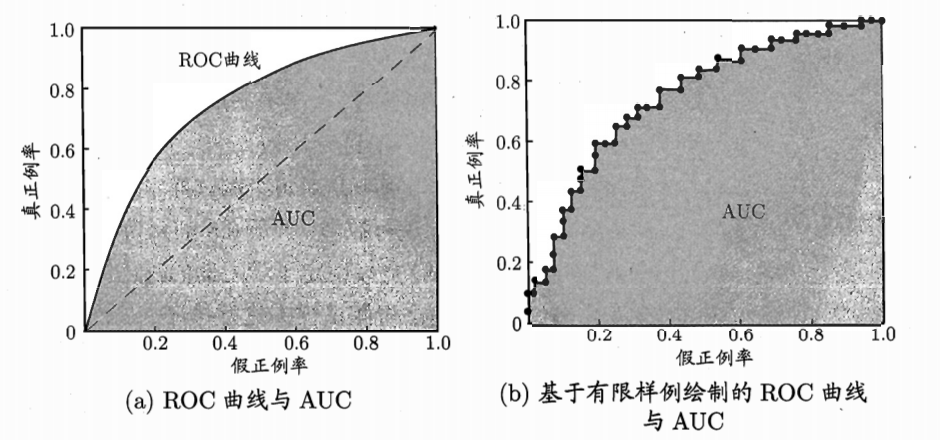
\includegraphics[scale=0.6]{../figures/RAMS3.PNG} 
\end{center}
若一个学习器的ROC曲线被另一个学习器的曲线完全“包住”,则可断言后者的性能优于前者。若两个学习器的ROC曲线有交叉点,则可比较ROC曲线下的面积,即AUC(Area Under ROC Curve)
\paragraph{AUC计算}假定ROC曲线是由坐标为$\{ (x_1,y_1),(x_2,y_2),\cdots,(x_m,y_m) \}$的点按序连接而形成(即$x_1=0,\cdots,x_m=1$),AUC可估算为
\begin{eqnarray}
AUC=\frac{1}{2}\sum_{i=1}^{m-1}(x_{i+1}-x_i)\cdot(y_i+y_{i+1})
\end{eqnarray}
给定$m^+$个正例和$m^-$个反例,令$D^+$和$D^-$分别表示正、反例集合,则排序“损失”(loss)定义为
\begin{eqnarray}
l_{rank}=\frac{1}{m^+m^-}\sum_{x^+\in D^+}\sum_{x^-\in D^-}
\left(
	1(f(x^+)<f(x^-))+\frac{1}{2}1(f(x^+)=f(x^-))
\right)
\end{eqnarray}

即考虑每一个正、反例,若正例的预测值小于反例,在记1个“罚分”,若相等,则记0.5个“罚分”。易得,$l_{rank}$对应的是ROC曲线之上的面积,若一个正例在ROC曲线上对应标记点的坐标为$(x,y)$,则$x$恰是排序在其之前的反例所占的比例,即假正例率,因此有
\begin{eqnarray}
AUC=1-l_{rank}
\end{eqnarray}

\subsubsection{代价敏感错误率与代价曲线}
以二分类为例,定义代价矩阵(cross matrix),其中$cost_{ij}$为第$i$类样本预测为第$j$类样本的代价。若将第0类判别为第1类所造成的损失更大,则$cost_{01}>cost_{10}$。代价矩阵如下
\begin{center}
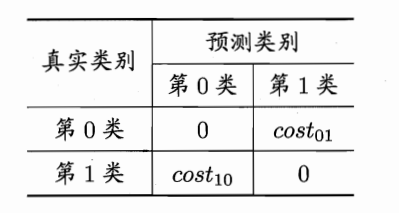
\includegraphics[scale=0.7]{../figures/RAMS4.PNG} 
\end{center}

在非均等代价下,目标不再是简单地最小化错误次数,而是最小化“总体代价”(total cost)







\subsection{特征选择}
对于一个有监督学习问题,数据的特征$n$很大,有可能为$n\gg m$,但是其中只有一小部分的特征是和学习任务相关的。当对$n$维的输入特征用简单的线性分类时,假设类的VC维将会是$O(n)$的,当训练数据不够大时,则过拟合是一个潜在的问题。于是,可以考虑采用特征选择算法来降低特征的数量。

\subsubsection{封装模型特征选择}
对于给定的$n$个特征,存在有$2^n$的可能的特征子集(因为特征有可能包含或不包含在子集中),因此特征选择转化为在$2^n$个可能的模型中的模型选择问题。对于一个很大的值$n$,计算和比较这$2^n$个模型将会变得很昂贵,所以采用启发式搜索的方法来寻找好的特征子集。这个搜索方法被称为前向搜索(forward search):
\begin{enumerate}[1]
\item 初始化$\mathcal{F}=\emptyset$
\item Repeat$\{$\\
\indent \ \ For $i=1,\cdots,n$\\
\indent \ \ \ \ (a)若$i\notin \mathcal{F}$,则令$\mathcal{F}_i=\mathcal{F}\cup\{i\}$,然后应用交叉验证的方法来评估特征$\mathcal{F}_i$(只使用$\mathcal{F}_i$中的特征来训练模型,并估计其泛化误差)
\\
\indent \ \ \ \ (b)将$\mathcal{F}$设为(a)中所找到的最优的特征子集$\}$
\item 经过如上循环而得到的最优特征子集。
\end{enumerate}

当$\mathcal{F}=\{1,2,\cdots,n\}$包含了所有的特征,或$\mathcal{F}$包含的特征数$\mathcal{F}$达到了一定的阈值(假设对特征数设置了最大值),算法的最外层循环将会终止。

上述的算法称为封装模型特征选择算法(wrapper model feature selection algorithm)。其含义是,我们“封装”了我们的算法模型,然后用不同的特征子集来估计算法的效果。除了前向搜索方法外,还有后向搜索方法,其与前项搜索方法的区别在于,其从$\mathcal{F}=\{1,2,\cdots,n\}$(包含所有特征)开始,然后重复删去特征,直到达到循环终止条件或$\mathcal{F}=\emptyset$。

封装模型特征选择算法通常情况下有好的效果,但是其多次调用学习算法会增大计算成本。实际上,完整的前向搜索算法,将会调用学习算法的次数为$O(n^2)$。

\subsubsection{过滤特征选择}
过滤特征选择提供了一种计算成本更小的选择特征子集的启发式算法。其思路是计算得分$S(i)$来度量特征$x_i$对类标签$y$的信息量。之后,只需找出$k$个得分最大的$S(i)$所对应的特征$i$。

一种定义$S(i)$的方式是基于训练集,计算$x_i$和$y$的协方差的绝对值,之后选择协方差绝对值大的几个特征作为最优特征子集。但有一种选择$S(i)$的更加常见的方法(尤其针对特征$x_i$为离散变量)为$x_i$和$y$之间的互信息(mutual information)$MI(x_i,y)$
\begin{eqnarray}
MI(x_i,y)=\sum_{x_i\in\{0,1\}}\sum_{y\in\{0,1\}}p(x_i,y)\log\frac{p(x_i,y)}{p(x_i)p(y)}
\end{eqnarray}
以上的方程假设$x_i$和$y_i$为二元分布。概率$P(x_i,y)$,$p(x_i)$,$p(y)$可以根据训练集的经验分布来估计。其也可以用KL散度(KUllback-leibler(KL)divergence)来表示
\begin{eqnarray}
MI(x_i,y)=KL(p(x_i,y)||p(x_i)p(y))
\end{eqnarray}

相对熵,又称为KL散度,是描述两个概率分布$P$和$Q$差异的一种方法,它是非对称的,这意味着$D(P||Q)\neq D(Q||P)$。在信息论中,$D(P||Q)$表示当用概率分布$Q$来拟合真实分布$P$时,产生的信息损耗,其中$P$表示真实分布,$Q$表示拟合分布。

设$P(x)$和$Q(x)$是$X$取值的两个离散概率分布,则$P$对$Q$的相对熵为
\begin{eqnarray}
D(P||Q)=\sum P(x)\log\frac{P(x)}{Q(x)}
\end{eqnarray}

于是,其给出了一种度量两个分布不同的方法。若$x_i$和$y$是独立随机变量,则有$p(x_i,y)=p(x_i)p(y)$,则这两个变量对应的分布的KL散度为0。因而若$x_i$和$y$是相互独立的,则可视为“$x_i$对$y$没有信息量”,因而得分$S(i)$很小。相反,若“$x_i$对$y$有信息量”,则其互信息$MI(x_i,y)$将是大的。

若已经根据得分$S(i)$对特征进行排序了,那么如何确定要选择的特征数目$k$?一种常规的方法是用交叉验证,在可能的值中选择$k$。例如,当利用朴素贝叶斯进行文本分类时,词汇量$n$通常会很大,使用这个方法来选择特征子集,将能够提高分类准确率。

\subsection{贝叶斯统计与规范化}
下面介绍一种用来克服过拟合的工具。我们采用最大化似然(maximum likelihood)来拟合参数,有
\begin{eqnarray}
\theta_{ML}=\arg\max_\theta\prod_{i=1}^mp(\sample{y}{i}|\sample{x}{i};\theta)
\end{eqnarray}
我们将$\theta$看作未知的参数。将$\theta$视为未知的但固定的参数是采用了频率学派统计学(frequentist statistics)的观点。在这个观点中,$\theta$不是随机的,只是其是未知的,于是我们的任务是通过统计学的方法(像极大似然估计)来估计参数。

另一种解决参数估计问题的方法是采用贝叶斯学派(Bayesian)的观点,然后把$\theta$视为一个随机变量。在这个方法中,我们对$\theta$确定一个先验分布(prior distribution)$p(\theta)$,来表达参数的先验信念(prior belief)。对于给定的训练集$S=\{ (\sample{x}{i},\sample{y}{i}) \}^m_{i=1}$当要对新的值$x$做预测时,我们可以先计算其后验分布(posterior distribution)
\begin{eqnarray}
\begin{aligned}
p(\theta|S)&=\frac{p(S|\theta) p(\theta)}{p(S)}\\
&= \frac{(\prod_{i=1}^mp(\sample{y}{i}|\sample{x}{i},\theta))p(\theta)}{\int_\theta (\prod_{i=1}^mp(\sample{y}{i}|\sample{x}{i},\theta)p(\theta))d\theta }
\end{aligned}
\end{eqnarray}
在上面的等式中,$p(\sample{y}{i}|\sample{x}{i},\theta)$来自所使用的模型。例如,若使用贝叶斯逻辑斯蒂回归,当$h_\theta(\sample{x}{i})=\frac{1}{1+e^{-\theta^T\sample{x}{i}}}$
则会选择$p(\sample{y}{i}|\sample{x}{i},\theta)=h_{\theta}(\sample{x}{i})^{\sample{y}{i}}(1-h_\theta (\sample{x}{i}))^{1-\sample{y}{i}}$

对于一个新的测试样例$x$,我们将用它做预测,我们可以基于在$\theta$的后延分布来计算在训练标签上的后验分布
\begin{eqnarray}
p(y|x,S)=\int_\theta p(y|x,\theta)p(\theta|S)d\theta
\end{eqnarray}
其中,$p(\theta|S)$来自上面,因此若目标是基于$x$来预测$y$,则可以得到
\begin{eqnarray}
E[y|x,S]=\int_yyp(y|x,S)dy
\end{eqnarray}
这个方法可以被视为 “完全贝叶斯(fully Bayesian)”预测。但实际上,后验分布很难计算,因为在求$p(\theta|S)$和计算后验概率时,需要完整的$\theta$的情况,因此其不可能算出解析解。

因此对$\theta$进行估计。一种方法是用点估计代替后验分布。用最大后验概率(maximum a posteriori)来估计$\theta$如下
\begin{eqnarray}
\theta_{MAP}=\arg\max_\theta\prod_{i=1}^mp(\sample{y}{i}|\sample{x}{i},\theta)p(\theta)
\end{eqnarray}
这个形式与对$\theta$最大似然估计相似,除了最后一项$p(\theta)$。

在应用中,可以将先验概率$p(\theta)$假设为服从$\theta\sim\mathcal{N}(0,\tau^2I)$。选择这种先验概率,拟合的参数$\theta_{MAP}$将会比使用最大似然要小,这也让贝叶斯MAP估计要比最大似然估计不容易过拟合。例如,贝叶斯逻辑斯蒂回归在文本分类上是一种高效的做法,虽然在文本分类中,通常会有$n\gg m$。








